\section{Оценка качества синтеза}
	После обучения сети, необходимо проверить, что сгенерированные ей изображения действительно имеют искомые характеристики. Для этого нужно ввести специальную метрику, которая будет учитывать наличие в изображении тренда интенсивности частиц. Было решено использовать среднюю плотность черных пикселей в некотором окне, и проходить этим окном по изображению (Рис. \ref{window}):
	\newpage
	$$\xi_k = \frac{1}{H w}{\sum_{i=k}^{k+w} \sum_{j=0}^{H}\left| \frac{x(i, j) - 255}{255} \right|}, $$$$k = \overline{1, W - w + 1} $$
	\begin{figure}
		\centering{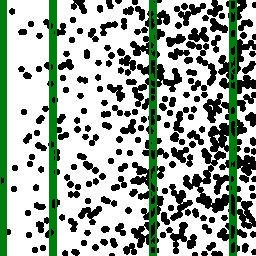
\includegraphics[width=0.35\linewidth]{metrics}}
		\caption{Прохождение окном, W, H - размеры изображения, w - ширина окна.}
		\label{window}
	\end{figure}
	
	Построив график $\xi(k)$, можно увидеть, как меняется плотность пикселей и прослеживается ли тренд. В качестве метрики можно взять среднеквадратичную ошибку:
	$$ \xi = \frac{1}{W-w}\sum_{k=1}^{W-w+1} (\xi_k - \xi_{0k})^2,$$
	где $\xi_{0k}$ - это $\xi_k$, усредненное по примерам из обучающей выборки. Соответственно, чем меньше значение метрики, тем лучше тренд, присутствующий на сгенерированном изображении, приближает искомый.